\documentclass[border=12pt]{standalone}
\usepackage{tikz}
\usetikzlibrary{shapes.geometric, arrows.meta, positioning, calc, fit, backgrounds}
\usepackage{fontspec}
\setmainfont{DejaVu Sans}

\begin{document}
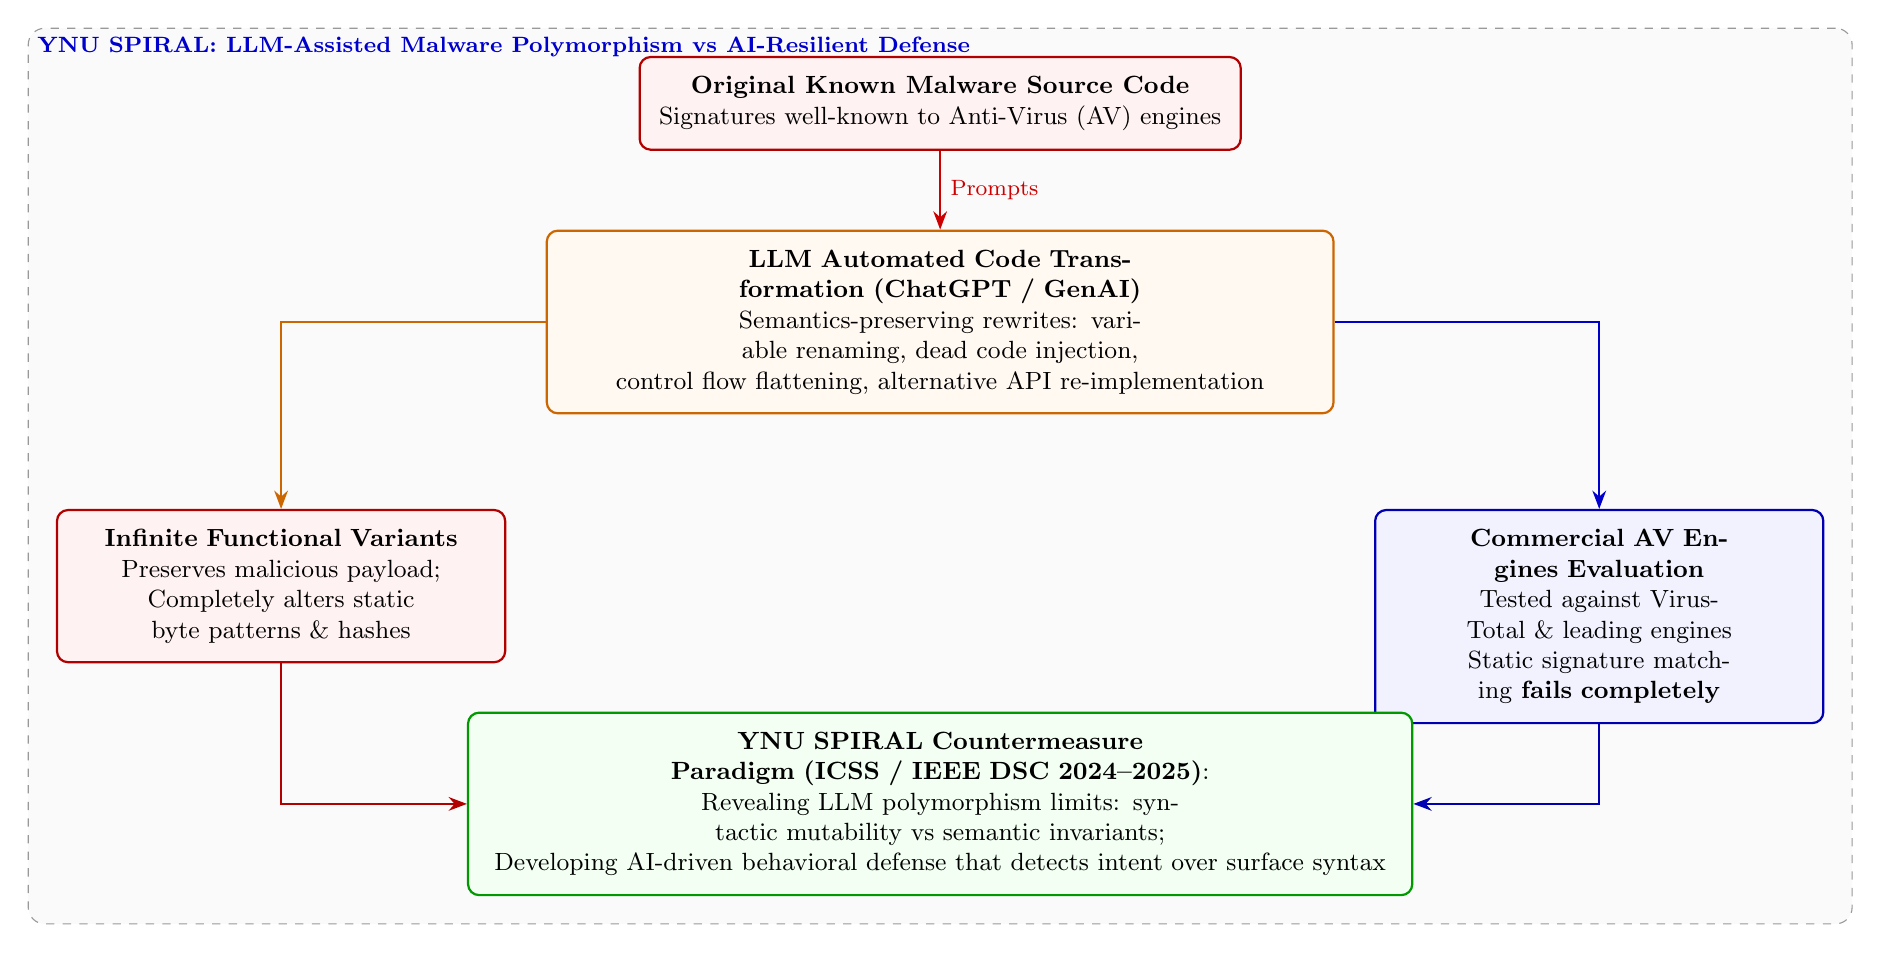
\begin{tikzpicture}[
    font=\small,
    >=Stealth,
    node distance=1.2cm,
    block/.style={rectangle, draw=blue!70!black, fill=blue!5, rounded corners=4pt, thick, align=center, inner sep=7pt},
    alertblock/.style={rectangle, draw=red!70!black, fill=red!5, rounded corners=4pt, thick, align=center, inner sep=7pt},
    greenblock/.style={rectangle, draw=green!60!black, fill=green!5, rounded corners=4pt, thick, align=center, inner sep=7pt},
    amberblock/.style={rectangle, draw=orange!80!black, fill=orange!5, rounded corners=4pt, thick, align=center, inner sep=7pt},
    groupbox/.style={draw=black!40, dashed, rounded corners=6pt, fill=black!2, inner sep=10pt}
]

    % Top Node: Known Malware Source Code
    \node[alertblock] (source) {\textbf{Original Known Malware Source Code}\\Signatures well-known to Anti-Virus (AV) engines};

    % Central Process: LLM Automated Metamorphism
    \node[amberblock, below=1.0cm of source, text width=9.5cm] (chatgpt) {\textbf{LLM Automated Code Transformation (ChatGPT / GenAI)}\\Semantics-preserving rewrites: variable renaming, dead code injection,\\control flow flattening, alternative API re-implementation};
    \draw[->, thick, red!80!black] (source) -- node[right, font=\footnotesize] {Prompts} (chatgpt);

    % Two Branches: Generated Variants vs Traditional AV Engines
    \node[alertblock, below left=1.2cm and 0.5cm of chatgpt, text width=5.2cm] (variants) {\textbf{Infinite Functional Variants}\\Preserves malicious payload;\\Completely alters static byte patterns \& hashes};

    \node[block, below right=1.2cm and 0.5cm of chatgpt, text width=5.2cm] (avscan) {\textbf{Commercial AV Engines Evaluation}\\Tested against VirusTotal \& leading engines\\Static signature matching \textbf{fails completely}};

    \draw[->, thick, orange!80!black] (chatgpt) -| (variants);
    \draw[->, thick, blue!80!black] (chatgpt) -| (avscan);

    % Bottom Synthesis: YNU SPIRAL Academic Defense
    \node[greenblock, below=1.4cm of $(variants)!0.5!(avscan)$, text width=11.5cm] (defense) {\textbf{YNU SPIRAL Countermeasure Paradigm (ICSS / IEEE DSC 2024--2025)}:\\Revealing LLM polymorphism limits: syntactic mutability vs semantic invariants;\\Developing AI-driven behavioral defense that detects intent over surface syntax};

    \draw[->, thick, red!70!black] (variants) |- (defense);
    \draw[->, thick, blue!70!black] (avscan) |- (defense);

    \begin{scope}[on background layer]
        \node[groupbox, fit=(source) (chatgpt) (variants) (avscan) (defense), label={[anchor=north west, font=\footnotesize\bfseries, blue!80!black]north west:YNU SPIRAL: LLM-Assisted Malware Polymorphism vs AI-Resilient Defense}] {};
    \end{scope}

\end{tikzpicture}
\end{document}
